\documentclass{ximera}

%\usepackage{todonotes}

\newcommand{\todo}{}

\usepackage{esint} % for \oiint
\ifxake%%https://math.meta.stackexchange.com/questions/9973/how-do-you-render-a-closed-surface-double-integral
\renewcommand{\oiint}{{\large\bigcirc}\kern-1.56em\iint}
\fi


\graphicspath{
  {./}
  {ximeraTutorial/}
  {basicPhilosophy/}
  {functionsOfSeveralVariables/}
  {normalVectors/}
  {lagrangeMultipliers/}
  {vectorFields/}
  {greensTheorem/}
  {shapeOfThingsToCome/}
  {dotProducts/}
  {partialDerivativesAndTheGradientVector/}
  {../productAndQuotientRules/exercises/}
  {../normalVectors/exercisesParametricPlots/}
  {../continuityOfFunctionsOfSeveralVariables/exercises/}
  {../partialDerivativesAndTheGradientVector/exercises/}
  {../directionalDerivativeAndChainRule/exercises/}
  {../commonCoordinates/exercisesCylindricalCoordinates/}
  {../commonCoordinates/exercisesSphericalCoordinates/}
  {../greensTheorem/exercisesCurlAndLineIntegrals/}
  {../greensTheorem/exercisesDivergenceAndLineIntegrals/}
  {../shapeOfThingsToCome/exercisesDivergenceTheorem/}
  {../greensTheorem/}
  {../shapeOfThingsToCome/}
  {../separableDifferentialEquations/exercises/}
  {vectorFields/}
}

\newcommand{\mooculus}{\textsf{\textbf{MOOC}\textnormal{\textsf{ULUS}}}}

\usepackage{tkz-euclide}
\usepackage{tikz}
\usepackage{tikz-cd}
\usetikzlibrary{arrows}
\tikzset{>=stealth,commutative diagrams/.cd,
  arrow style=tikz,diagrams={>=stealth}} %% cool arrow head
\tikzset{shorten <>/.style={ shorten >=#1, shorten <=#1 } } %% allows shorter vectors

\usetikzlibrary{backgrounds} %% for boxes around graphs
\usetikzlibrary{shapes,positioning}  %% Clouds and stars
\usetikzlibrary{matrix} %% for matrix
\usepgfplotslibrary{polar} %% for polar plots
\usepgfplotslibrary{fillbetween} %% to shade area between curves in TikZ
%\usetkzobj{all}
\usepackage[makeroom]{cancel} %% for strike outs
%\usepackage{mathtools} %% for pretty underbrace % Breaks Ximera
%\usepackage{multicol}
\usepackage{pgffor} %% required for integral for loops



%% http://tex.stackexchange.com/questions/66490/drawing-a-tikz-arc-specifying-the-center
%% Draws beach ball
\tikzset{pics/carc/.style args={#1:#2:#3}{code={\draw[pic actions] (#1:#3) arc(#1:#2:#3);}}}



\usepackage{array}
\setlength{\extrarowheight}{+.1cm}
\newdimen\digitwidth
\settowidth\digitwidth{9}
\def\divrule#1#2{
\noalign{\moveright#1\digitwidth
\vbox{\hrule width#2\digitwidth}}}




% \newcommand{\RR}{\mathbb R}
% \newcommand{\R}{\mathbb R}
% \newcommand{\N}{\mathbb N}
% \newcommand{\Z}{\mathbb Z}

\newcommand{\sagemath}{\textsf{SageMath}}


%\renewcommand{\d}{\,d\!}
%\renewcommand{\d}{\mathop{}\!d}
%\newcommand{\dd}[2][]{\frac{\d #1}{\d #2}}
%\newcommand{\pp}[2][]{\frac{\partial #1}{\partial #2}}
% \renewcommand{\l}{\ell}
%\newcommand{\ddx}{\frac{d}{\d x}}

% \newcommand{\zeroOverZero}{\ensuremath{\boldsymbol{\tfrac{0}{0}}}}
%\newcommand{\inftyOverInfty}{\ensuremath{\boldsymbol{\tfrac{\infty}{\infty}}}}
%\newcommand{\zeroOverInfty}{\ensuremath{\boldsymbol{\tfrac{0}{\infty}}}}
%\newcommand{\zeroTimesInfty}{\ensuremath{\small\boldsymbol{0\cdot \infty}}}
%\newcommand{\inftyMinusInfty}{\ensuremath{\small\boldsymbol{\infty - \infty}}}
%\newcommand{\oneToInfty}{\ensuremath{\boldsymbol{1^\infty}}}
%\newcommand{\zeroToZero}{\ensuremath{\boldsymbol{0^0}}}
%\newcommand{\inftyToZero}{\ensuremath{\boldsymbol{\infty^0}}}



% \newcommand{\numOverZero}{\ensuremath{\boldsymbol{\tfrac{\#}{0}}}}
% \newcommand{\dfn}{\textbf}
% \newcommand{\unit}{\,\mathrm}
% \newcommand{\unit}{\mathop{}\!\mathrm}
% \newcommand{\eval}[1]{\bigg[ #1 \bigg]}
% \newcommand{\seq}[1]{\left( #1 \right)}
% \renewcommand{\epsilon}{\varepsilon}
% \renewcommand{\phi}{\varphi}


% \renewcommand{\iff}{\Leftrightarrow}

% \DeclareMathOperator{\arccot}{arccot}
% \DeclareMathOperator{\arcsec}{arcsec}
% \DeclareMathOperator{\arccsc}{arccsc}
% \DeclareMathOperator{\si}{Si}
% \DeclareMathOperator{\scal}{scal}
% \DeclareMathOperator{\sign}{sign}


%% \newcommand{\tightoverset}[2]{% for arrow vec
%%   \mathop{#2}\limits^{\vbox to -.5ex{\kern-0.75ex\hbox{$#1$}\vss}}}
% \newcommand{\arrowvec}[1]{{\overset{\rightharpoonup}{#1}}}
% \renewcommand{\vec}[1]{\arrowvec{\mathbf{#1}}}
% \renewcommand{\vec}[1]{{\overset{\boldsymbol{\rightharpoonup}}{\mathbf{#1}}}}

% \newcommand{\point}[1]{\left(#1\right)} %this allows \vector{ to be changed to \vector{ with a quick find and replace
% \newcommand{\pt}[1]{\mathbf{#1}} %this allows \vec{ to be changed to \vec{ with a quick find and replace
% \newcommand{\Lim}[2]{\lim_{\point{#1} \to \point{#2}}} %Bart, I changed this to point since I want to use it.  It runs through both of the exercise and exerciseE files in limits section, which is why it was in each document to start with.

% \DeclareMathOperator{\proj}{\mathbf{proj}}
% \newcommand{\veci}{{\boldsymbol{\hat{\imath}}}}
% \newcommand{\vecj}{{\boldsymbol{\hat{\jmath}}}}
% \newcommand{\veck}{{\boldsymbol{\hat{k}}}}
% \newcommand{\vecl}{\vec{\boldsymbol{\l}}}
% \newcommand{\uvec}[1]{\mathbf{\hat{#1}}}
% \newcommand{\utan}{\mathbf{\hat{t}}}
% \newcommand{\unormal}{\mathbf{\hat{n}}}
% \newcommand{\ubinormal}{\mathbf{\hat{b}}}

% \newcommand{\dotp}{\bullet}
% \newcommand{\cross}{\boldsymbol\times}
% \newcommand{\grad}{\boldsymbol\nabla}
% \newcommand{\divergence}{\grad\dotp}
% \newcommand{\curl}{\grad\cross}
%\DeclareMathOperator{\divergence}{divergence}
%\DeclareMathOperator{\curl}[1]{\grad\cross #1}
% \newcommand{\lto}{\mathop{\longrightarrow\,}\limits}

% \renewcommand{\bar}{\overline}

\colorlet{textColor}{black}
\colorlet{background}{white}
\colorlet{penColor}{blue!50!black} % Color of a curve in a plot
\colorlet{penColor2}{red!50!black}% Color of a curve in a plot
\colorlet{penColor3}{red!50!blue} % Color of a curve in a plot
\colorlet{penColor4}{green!50!black} % Color of a curve in a plot
\colorlet{penColor5}{orange!80!black} % Color of a curve in a plot
\colorlet{penColor6}{yellow!70!black} % Color of a curve in a plot
\colorlet{fill1}{penColor!20} % Color of fill in a plot
\colorlet{fill2}{penColor2!20} % Color of fill in a plot
\colorlet{fillp}{fill1} % Color of positive area
\colorlet{filln}{penColor2!20} % Color of negative area
\colorlet{fill3}{penColor3!20} % Fill
\colorlet{fill4}{penColor4!20} % Fill
\colorlet{fill5}{penColor5!20} % Fill
\colorlet{gridColor}{gray!50} % Color of grid in a plot

\newcommand{\surfaceColor}{violet}
\newcommand{\surfaceColorTwo}{redyellow}
\newcommand{\sliceColor}{greenyellow}




\pgfmathdeclarefunction{gauss}{2}{% gives gaussian
  \pgfmathparse{1/(#2*sqrt(2*pi))*exp(-((x-#1)^2)/(2*#2^2))}%
}


%%%%%%%%%%%%%
%% Vectors
%%%%%%%%%%%%%

%% Simple horiz vectors
\renewcommand{\vector}[1]{\left\langle #1\right\rangle}


%% %% Complex Horiz Vectors with angle brackets
%% \makeatletter
%% \renewcommand{\vector}[2][ , ]{\left\langle%
%%   \def\nextitem{\def\nextitem{#1}}%
%%   \@for \el:=#2\do{\nextitem\el}\right\rangle%
%% }
%% \makeatother

%% %% Vertical Vectors
%% \def\vector#1{\begin{bmatrix}\vecListA#1,,\end{bmatrix}}
%% \def\vecListA#1,{\if,#1,\else #1\cr \expandafter \vecListA \fi}

%%%%%%%%%%%%%
%% End of vectors
%%%%%%%%%%%%%

%\newcommand{\fullwidth}{}
%\newcommand{\normalwidth}{}



%% makes a snazzy t-chart for evaluating functions
%\newenvironment{tchart}{\rowcolors{2}{}{background!90!textColor}\array}{\endarray}

%%This is to help with formatting on future title pages.
\newenvironment{sectionOutcomes}{}{}



%% Flowchart stuff
%\tikzstyle{startstop} = [rectangle, rounded corners, minimum width=3cm, minimum height=1cm,text centered, draw=black]
%\tikzstyle{question} = [rectangle, minimum width=3cm, minimum height=1cm, text centered, draw=black]
%\tikzstyle{decision} = [trapezium, trapezium left angle=70, trapezium right angle=110, minimum width=3cm, minimum height=1cm, text centered, draw=black]
%\tikzstyle{question} = [rectangle, rounded corners, minimum width=3cm, minimum height=1cm,text centered, draw=black]
%\tikzstyle{process} = [rectangle, minimum width=3cm, minimum height=1cm, text centered, draw=black]
%\tikzstyle{decision} = [trapezium, trapezium left angle=70, trapezium right angle=110, minimum width=3cm, minimum height=1cm, text centered, draw=black]


\title{Analysis}

\begin{document}

\begin{abstract}
8 characteristics
\end{abstract}
\maketitle












Analyze $H(x) = 5 \sqrt{x^2-3}$ with its natural domain. \\



\subsection*{Analysis}




Our plan is to view this as a composition. \\






We are looking for functions $f$ and $g$ such that $(f \circ g)(x) = f(g(x)) = 5 \sqrt{x^2-3}$ \\


First, identify ``insides'' of functions.  In this case, $x^2 - 3$ is the inside of $5 \sqrt{t}$. \\



\begin{itemize}
\item Let $f(t) = 5 \sqrt{t}$ \\
\item Let $g(y) = y^2 - 3$ \\
\end{itemize}

Algebraically, this produces the formula want, $(f \circ g)(x) = f(g(x)) = 5 \sqrt{x^2-3}$.

To get us started, we are thinking that each component function comes with its natural domain.

\begin{itemize}
\item Let $f(t) = 5 \sqrt{t}$ with domain $[0, \infty)$ \\
\item Let $g(y) = y^2 - 3$ with domain $(-\infty, \infty)$ \\
\end{itemize}

We are also ready to revise and modify and restrict these domains to fit the composition together. \\





We are ready to analyze. \\




\textbf{\textcolor{blue!55!black}{Domain:}} \\


$H$ is not a square root function, since the inside is not a linear function.  However, the formula includes a square root and the inside of it must not be negative. \\

We need $x^2-3 \geq 0$.  Therefore, the domain of $H$ is is the part of the domain of $g$ that is in common (intersects) with $(-\infty, -\sqrt{3} ] \cup [ \sqrt{3}, \infty)$. \\

Since, the natural domainm of $g$ is $(-\infty, \infty)$, the domain of $H$ is also $(-\infty, -\sqrt{3} ] \cup [ \sqrt{3}, \infty)$. \\



\textbf{\textcolor{blue!55!black}{Zeros:}} \\


The zeros of $H$ are the domain numbers of $H$ where $H$ equals $0$.  This would be where $f = 0$, since the values of $H$ are values of $f$. \\



$f(t) = \sqrt{t}$ equals $0$ when $t = 0$. Therefore, we are looking for when the output of $g$ equals $0$. \\



$g(y) = y^2 - 3 = 0$ at $-\sqrt{3}$ and $\sqrt{3}$. \\



Or, we could just work with the entire formula for $H$. \\


\[
5 \sqrt{x^2-3} = 0
\]


\[
\sqrt{x^2-3} = 0
\]


\[
x^2-3 = 0
\]

\[
x^2 = 3
\]


We have two zeros, $-\sqrt{3}$ and $\sqrt{3}$. \\

We just have to make sure these are actually in the domain of $H$.  They are. \\






\textbf{\textcolor{blue!55!black}{Continuity:}} \\


$H$ is a composition of a root function and a quadratic funciton.  Both of these are continuous, which means their composition is continuous. \\

Neither root functions nor quadratics have discontinuites or singularities. \\





\textbf{\textcolor{blue!55!black}{End-Behavior:}} \\



We'll think of this in two steps. First, we'll determine the end-behavior of $g$, then we'll determine the end-behavior of $f$ with respect to the end-behavior of $g$.\\


Since $g$ is a quadratic function with a negative leading coefficient, we know that 

\[
\lim\limits_{y \to -\infty} g(y) = \lim\limits_{y \to -\infty} (y^2 - 3)  = \infty
\]


\[
\lim\limits_{y \to \infty} g(y) = \lim\limits_{y \to \infty} (y^2 - 3)  = \infty
\]

This means the limit of $H$ is the limit of $f$ as the domain of $f$ approaches $\infty$. \\


$f$ is a square root function with positive leading coefficients inside and out. \\

\[
\lim\limits_{x \to -\infty} H(x) =  \lim\limits_{t \to \infty} f(t)  = \lim\limits_{t \to \infty} 5\sqrt{t} = \infty
\]


\[
\lim\limits_{x \to \infty} H(x) =  \lim\limits_{t \to \infty} f(t)  = \lim\limits_{t \to \infty} 5\sqrt{t} = \infty
\]









\textbf{\textcolor{blue!55!black}{Behavior:}} \\


We want to figure out where $H$ is increasing and decreasing. \\

$H$ is a composition, so we need to know how the component functions behave. \\





$f(t) = 5 \sqrt{t}$ is an increasing function, since it is a root function with positive leading coefficients inside and outside. \\

$g(y) = y^2 - 3$ is a quadratic with a positive leading coefficient.  Therefore, it decreases and then increases.   It switches at its criticial number.\\



\[
\frac{-b}{2 a} = \frac{0}{2} = 0
\]


$g$ decreases on $(-\infty, 0)$ and increases on $(0, \infty)$.  However, $0$ is not in the domain of $H$. We need to restrict this information to the actual domain of $H$. \\





\textbf{\textcolor{blue!55!black}{blacktriangleright}} On $(-\infty, -\sqrt{3}]$, 


$g$ is decreasing. Here, the range of $g$ is positive and $f$ is increasing for positive domain numbers. \\ 



\begin{center}
$H$ is $increasing \circ decreasing$, which is decreasing. \\
\end{center}





\textbf{\textcolor{blue!55!black}{blacktriangleright}} On $[\sqrt{3}, \infty)$, 


$g$ is increasing. Here, the range of $g$ is positive and $f$ is increasing for positive domain numbers. \\ 


\begin{center}
$H$ is $increasing \circ increasing$, which is increasing. \\
\end{center}













\textbf{\textcolor{blue!55!black}{Local Maximum and Minimum:}} \\





On $(-\infty, -\sqrt{3} ]$, $H$ is $decreasing$, which makes $H(-\sqrt{3}) = 0$ a local minimum.  \\


On $[ \sqrt{3}, \infty)$, $H$ is $increasing$, which makes $H(\sqrt{3}) = 0$ a local minimum.  \\



There are no other critical numbers or endpoints in the domain.









\textbf{\textcolor{blue!55!black}{Global Maximum and Minimum:}} \\



On $(-\infty, -\sqrt{3} ]$, $H$ is $decreasing$, which makes $H(-\sqrt{3}) = 0$ a local minimum. \\


On $[ \sqrt{3}, \infty)$, $H$ is $increasing$, which makes $H(\sqrt{3}) = 0$ a local minimum  \\




Since $5 \sqrt{x^2-3} \geq 0$, $0$ is the global minimum. \\



$0$ is the global minimum value of $H$. It occurs at two places in the domain, $-\sqrt{3}$ and $\sqrt{3}$. \\



Since, $\lim\limits_{x \to -\infty} H(x) = \infty$, there is no global maximum. 














\textbf{\textcolor{blue!55!black}{Range:}} \\



$H$ is continuous and decreasing on $( -\infty, -\sqrt{3} ]$. \\


$\lim\limits_{x \to -\infty} H(x) = \infty$ \\


$H(-\sqrt{3}) = 0$


Therefore, the range of $H$ on $( -\infty, -\sqrt{3} ]$ is $[0, \infty)$. \\





$H$ is continuous and increasing on $[ \sqrt{3} ,\infty)$. \\


$\lim\limits_{x \to \infty} H(x) = \infty$ \\


$H(\sqrt{3}) = 0$


Therefore, the range of $H$ on $[ \sqrt{3}, \infty )$ is $[0, \infty)$. \\








The range of $H$ is $[0, \infty) \cup [0, \infty) = [0, \infty)$.




This all agrees with the graph. \\





\begin{image}
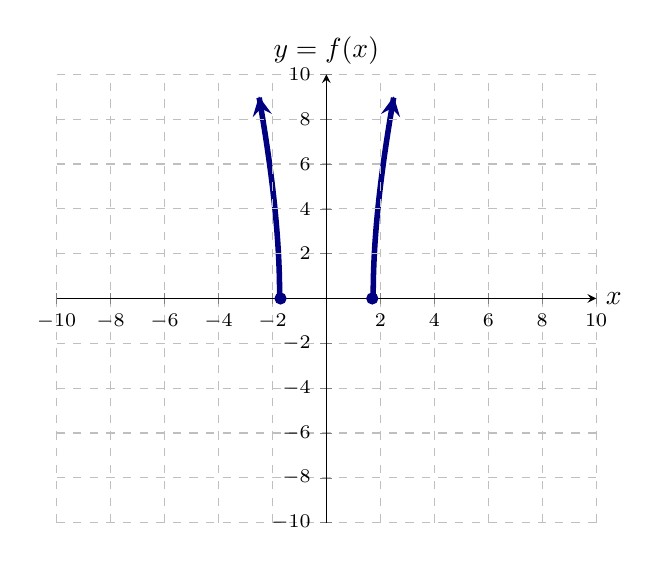
\begin{tikzpicture}
    \begin{axis}[name = sinax, domain=-10:10, ymax=10, xmax=10, ymin=-10, xmin=-10,
            axis lines =center, xlabel=$x$, ylabel={$y=f(x)$}, grid = major, grid style={dashed},
            ytick={-10,-8,-6,-4,-2,2,4,6,8,10},
            xtick={-10,-8,-6,-4,-2,2,4,6,8,10},
            yticklabels={$-10$,$-8$,$-6$,$-4$,$-2$,$2$,$4$,$6$,$8$,$10$}, 
            xticklabels={$-10$,$-8$,$-6$,$-4$,$-2$,$2$,$4$,$6$,$8$,$10$},
            ticklabel style={font=\scriptsize},
            every axis y label/.style={at=(current axis.above origin),anchor=south},
            every axis x label/.style={at=(current axis.right of origin),anchor=west},
            axis on top
          ]
          
          \addplot [line width=2, penColor, smooth,samples=100,domain=(-2.5:-1.7),<-] ({x},{5*sqrt(x^2 - 3)});
          \addplot [color=penColor,only marks,mark=*] coordinates{(-1.7,0)};


          \addplot [line width=2, penColor, smooth,samples=100,domain=(1.7:2.5),->] ({x},{5*sqrt(x^2 - 3)});
          \addplot [color=penColor,only marks,mark=*] coordinates{(1.7,0)};

           

    \end{axis}

\end{tikzpicture}
\end{image}

































\begin{center}
\textbf{\textcolor{green!50!black}{ooooo-=-=-=-ooOoo-=-=-=-ooooo}} \\

more examples can be found by following this link\\ \link[More Examples of Composition]{https://ximera.osu.edu/csccmathematics/precalculus2/precalculus2/composition/examples/exampleList}

\end{center}







\end{document}
